% This is auto-generated file: do not edit!
% Exported from microMathematics Plus, version 2.15.5


Diese App ist eine leistungsstarke
Rechensoftware im Arbeitsblatt Format.
Das Arbeitsblatt kann frei editiert,
auf einer SD Karte gespeichert werden,
von einer SD Karte aus geöffnet oder
in ein Bild- oder LaTeX-Format
exportiert werden. Es ermöglicht die
sofortige Bearbeitung von eingesetzten
mathematischen Bezeichnungen sowie
deren automatische Berechnung.

Die folgenden Objekte stehen zur
Verfügung: Gleichungen,
Ergebnisansichten, graphische
Darstellungen, Textfragmente und
Bilder. Diese Broschüre gibt Ihnen
einen Überblick darüber, wie man diese
Objekte erstellen und bearbeiten kann.

\subsection{Bearbeitung}

Fast alle Objekte bestehen aus frei
editierbaren Feldern. Um das Feld zu
bearbeiten, nutzen Sie die Symbole und
Funktionen der Werkzeugleiste.

Alle Symbole können auch über die
Tastatur eingefügt werden. Um
herauszufinden, welche Taste mit
welchem mathematischen Symbol
korrespondiert, lesen Sie den Hinweis
indem Sie den jeweiligen Button lange
gedrückt halten.

Langes Gedrückthalten eines Terms
erlaubt Ihnen, diesen Term
auszuwählen. Der ausgewählte Term kann
gelöscht, in die Zwischenablage
kopiert, von dort aus eingefügt
werden, oder eine Funktion oder ein
Symbol kann im Nachhinein von der
Werkzeugleiste oder Tastatur aus
eingefügt werden.

Sie können auch den ''Rückgängig''
Button in der Menüleiste benutzen, um
die letzte Eingabe rückgängig zu
machen:
\begin{center}\begin{tabular}{c} 
\includegraphics[resolution=320]{graphics/how_to_use_fig1.png} \end{tabular}\end{center}

\subsection{Gleichungen}

Eine Gleichung definiert eine
numerische Konstante, ein Intervall
oder eine Funktion. Um eine Gleichung
zu erstellen, nutzen Sie den ''Neu''
Button in der Menüleiste
\begin{center}\begin{tabular}{c} 
\includegraphics[resolution=320]{graphics/how_to_use_fig2.png} \end{tabular}\end{center}

oder den ''Gleichung hinzufügen'' Button
der Werkzeugleiste:
\begin{center}\begin{tabular}{c} 
\includegraphics[resolution=320]{graphics/how_to_use_fig3.png} \end{tabular}\end{center}

Eine Gleichung mit zwei lehren Feldern
wird erstellt:
\begin{center}\begin{tabular}{c}
  ${\Box} := {\Box}$
\end{tabular}\end{center}

Der Name der Gleichung muss in dem
linken Feld eingegeben sein. Der Name
darf nur Buchstaben und Zahlen
enthalten und wird in anderen
Gleichungen genutzt, um auf diese
Gleichung zu verweisen.

Sie können Menüleiste benutzen, um
''Dokumenteinstellungen'' Dialog zu
öffnen:
\begin{center}\begin{tabular}{c} 
\includegraphics[resolution=320]{graphics/how_to_use_fig4.png} \end{tabular}\end{center}

Abhängig vom Parameter ''Neubestimmung
erlauben'' in diesem Dialog sind zwei
Benutzungsmodi möglich:

a) Falls eine Neubestimmung nicht
erlaubt ist, bleibt die Gleichung
einzigartig im gesamten Arbeitsblatt
und die Gleichung kann sowohl vor als
auch nach ihrer Bestimmung verwendet
werden.

b) Falls eine Neubestimmung erlaubt
ist, können Sie mehr als eine
Gleichung mit dem selben Namen
bestimmen. Falls so eine Gleichung
dann referenziert wird, verwendet die
Software die zuletzt bestimmte
Version.

\subsubsection{Konstanten}

Falls der Name der Gleichung keine
Parameter in Klammern enthält,
definiert diese eine Konstante oder
ein Intervall:
\begin{center}\begin{tabular}{ccc}
  $N := 200$ &
  $Sq2 := \sqrt{100} $ &
  $Pi2 := \frac{{\pi}}{2}$ \cr
\end{tabular}\end{center}

In diesem Beispiel wurde die
integrierte Konstante Pi verwendet.
Aktuell sind folgende integrierte
Konstanten verfügbar: 
\begin{center}\begin{tabular}{ccc}
  ${\pi} = 3.14159$ &
  $pi = 3.14159$ &
  $e = 2.71828$ \cr
\end{tabular}\end{center}

Es kann auch eine zuvor definierte
Konstante verwendet werden: 
\begin{center}\begin{tabular}{c}
  $NPi2 := N \cdot Pi2$
\end{tabular}\end{center}

Eine komplexe Zahl als eine Konstante
wird durch zwei reele Zahlen und
imaginäre Einheit ''i'' definiert:
\begin{center}\begin{tabular}{c}
  $z := 5+3i$
\end{tabular}\end{center}

\subsubsection{Intervalle}

Eine Intervall-Gleichung definiert
eine Variable, die sich von einem
vorgegebenen Minimalwert in einem
vorgegebenem Schritte zu einem
vorgegebenen Maximalwert verändert.
Diese Variable kann als Parameter
genutzt werden, um eine
Funktionswert-Tabelle oder einen
Funktionsgraphen zu erstellen.

Um ein Intervall zu definieren, legen
Sie einen Namen auf der linken Seite
einer leeren Gleichung fest. Wählen
Sie auf der rechten Seite der
Gleichung entweder das Symbol '':'' oder
klicken Sie den Button ''Äquidistantes
Intervall'' in der Werkzeugleiste:
\begin{center}\begin{tabular}{c} 
\includegraphics[resolution=320]{graphics/how_to_use_fig5.png} \end{tabular}\end{center}

Das erste Element ist hier der
Anfangspunkt des Intervalls; das
nächste ist der zweite Punkt und das
letzte Element ist der Endpunkt des
Intervalls.
\begin{center}\begin{tabular}{c}
  $x := \left[ 0,\, 0.1 \,..\, 10 \right]$
\end{tabular}\end{center}

Man kann auf die Intervallemente
zugreiffen:
\begin{center}\begin{tabular}{ccc}
  $x \left( 0\right)  = 0.0$ &
  $x \left( 1\right)  = 0.1$ &
  $x \left( 100\right)  = 10.0$ \cr
\end{tabular}\end{center}

Der Abstand ist hier als Unterschied
zwischen dem zweiten und dem ersten
Wert gegeben:
\begin{center}\begin{tabular}{c}
  $x \left( 1\right)  - x \left( 0\right)  = 0.1$
\end{tabular}\end{center}

Beispielsweise können wir ein
äquidistantes Intervall definieren,
das bei Null beginnt und N Punkte mit
einem Abstand von ''dy'' hat:
\begin{center}\begin{tabular}{cc}
  $dy := 0.05$ &
  $y := \left[ 0,\, dy \,..\, dy \cdot N \right]$ \cr
\end{tabular}\end{center}

\subsubsection{Funktionen}

Eine Funktion ist eine Beziehung
zwischen zwei Mengen, die jedem
Element oder Wert der einen Menge
genau ein Element der anderen Menge
zuordnet.

Der Funktionsname und das
Funktionsargument in Klammern sind
links von der Gleichung zu finden. Das
Argument muss nicht zuvor im
Arbeitsblatt definiert worden sein.
Sie können es nach Belieben unter
Verwendung von Buchstaben und Zahlen
definieren:
\begin{center}\begin{tabular}{c}
  $f(t) := sin \left( t\right)  \cdot cos \left( t\right)  / 2$
\end{tabular}\end{center}
\begin{center}\begin{tabular}{c}
  $w(z) := {e}^{2i \cdot {\pi} \cdot z}$
\end{tabular}\end{center}
\begin{center}\begin{tabular}{c}
  $g(x,y) := \frac{sin \left( hypot \left( x,\, y\right) \right) }{hypot \left( x,\, y / 2\right)  + 1}$
\end{tabular}\end{center}

Rechts von der Funktion findet sich
eine mathematische Formel um die
Funktion zu berechnen. Falls diese
Formel das Funktionsargument nicht
enthält, wird diese Funktion als
Konstante interpretiert.

Sie können also in dieser Formel eine
integrierte oder zuvor definierte
Funktion einzufügen. Geben Sie dafür
einen Namen ein, klicken Sie auf das
linke Klammer-Symbol ''('' und wählen
Sie das Argument. Dies kann auch eine
Formel sein, die andere Operatoren
oder Funktionen enthält.

\subsubsection{Array}

Arrays sind besondere Funktionen, die
folgende Eigenschaften haben:

a) jedes Argument des Arrays muss ein
vorher definiertes Intervall sein:
\begin{center}\begin{tabular}{cc}
  $k := \left[ 0,\, 1 \,..\, 100 \right]$ &
  $m := \left[ 0,\, 1 \,..\, 200 \right]$ \cr
\end{tabular}\end{center}

a) die Argumente des Arrays sind in eckigen
Klammern ''[ ]'' anstelle der runden
Klammern ''( )'' geschrieben:
\begin{center}\begin{tabular}{c}
  $M[k,m] := {sin \left( k / 10\right) }^{2} - 3 \cdot  \left| cos \left( m / 10\right)  \right| $
\end{tabular}\end{center}

c) die Array-Elemente werden berechnet
und gespeichert. Dadurch ist der
Zugriff auf diese Elemente viel
schneller.

d) man kann die Array-Elemente nur
mittels eines Index zugreifen. Um
solchen Index zu erzeugen, geben Sie
''['' nach dem Array-Namen:
\begin{center}\begin{tabular}{cc}
  $M_{5,\, 10}  = -1.39106$ &
  $M_{10,\, 5}  = -1.92467$ \cr
\end{tabular}\end{center}
\begin{center}\begin{tabular}{c}
  $N[k,m] := floor \left( -10 \cdot M_{k,\, m} \right) $
\end{tabular}\end{center}

e) wenn ein Index ist komplex, negativ 
oder größer als die Obergrenze des
dazugehörigen Intervalls, dann wird
ein ungültigen Wert zurückgegeben:
\begin{center}\begin{tabular}{cc}
  $M_{10i,\, 100}  = NaN$ &
  $M_{90,\, 210}  = NaN$ \cr
\end{tabular}\end{center}

\subsection{Ergebnisansicht}

Dieses Element soll das Ergebnis einer
Berechnung als Zahl oder Tabelle
darstellen. Um eine Ergebnisansicht zu
erstellen, verwenden Sie den ''Neu''
Button in der Menüleiste oder
''Ergebnisansicht hinzufügen'' Button in
der Werkzeugleiste:
\begin{center}\begin{tabular}{c} 
\includegraphics[resolution=320]{graphics/how_to_use_fig6.png} \end{tabular}\end{center}

Eine Gleichung mit zwei lehren Feldern
wird erstellt:
\begin{center}\begin{tabular}{c}
  ${\Box} = {\Box}$
\end{tabular}\end{center}

Der linke Term enthält eine zu
berechnende Formel und der rechte Term
ist das Rechnungsergebnis. Hier können
Sie sämtliche zuvor bestimmten
Konstanten und Funktionen verwenden,
sowie alle integrierte Funktionen:
\begin{center}\begin{tabular}{c}
  ${e}^{{\pi}} \cdot f \left( NPi2\right)  = 2.27286E-14$
\end{tabular}\end{center}

Falls der linke Teil keine
''intervallähnlichen'' Variablen enthält
ist das Rechenergebnis nur eine reelle
oder komplexe Zahl.
\begin{center}\begin{tabular}{c}
  $y \left( N - 1\right)  - y \left( 0\right)  = 9.95$
\end{tabular}\end{center}
\begin{center}\begin{tabular}{ccc}
  $\Re\left( z \right)  = 5.0$ &
  $\Im\left( z \right)  = 3.0$ &
  $ \left| z \right|  = 5.83095$ \cr
\end{tabular}\end{center}
\begin{center}\begin{tabular}{c}
  $\sqrt{sin \left( \frac{3}{2} \cdot {\pi}\right) }  = 0.0+1.0i$
\end{tabular}\end{center}

Falls der linke Teil als Variable ein
Intervall enthält, ist das Ergebnis
ein Vektor von Werten, die dem
Intervall entsprechen. Aufgrund der
Platzbeschränkungen auf dem Display
werden nur die ersten sechs sowie das
letzte Element des Vektors angezeigt:
\begin{center}\begin{tabular}{ccc}
  $x = \begin{bmatrix}0.0\\0.1\\0.2\\0.3\\0.4\\0.5\\\dots\\10.0\\\end{bmatrix}$ &
  $y = \begin{bmatrix}0.0\\0.05\\0.1\\0.15\\0.2\\0.25\\\dots\\10.0\\\end{bmatrix}$ &
  $2 \cdot y = \begin{bmatrix}0.0\\0.1\\0.2\\0.3\\0.4\\0.5\\\dots\\20.0\\\end{bmatrix}$ \cr
\end{tabular}\end{center}
\begin{center}\begin{tabular}{c}
  $N_{k,\, m}  = \begin{bmatrix}30.0&29.0&29.0&28.0&\dots&12.0\\29.0&29.0&29.0&28.0&\dots&12.0\\29.0&29.0&29.0&28.0&\dots&11.0\\29.0&28.0&28.0&27.0&\dots&11.0\\\dots&\dots&\dots&\dots&\dots&\dots\\27.0&26.0&26.0&25.0&\dots&9.0\\\end{bmatrix}$
\end{tabular}\end{center}

Sie können die Anzahl der angezeigten
Elemente und die Darstellungsart der
Ergebnisse ändern. Halten Sie auf dem
linken Abschnitt lange gedrückt und
selektieren Sie mittels Kontextmenü
die komplette Formel. Wenn die Formel
markiert ist, erscheint ein Action
Button ''Objekteinstellungen''. Ein Tap
auf diesen Button öffnet das
Dialogfenster ''Ergebnisansicht'' mit
diesen Einstellungen:
\begin{center}\begin{tabular}{c} 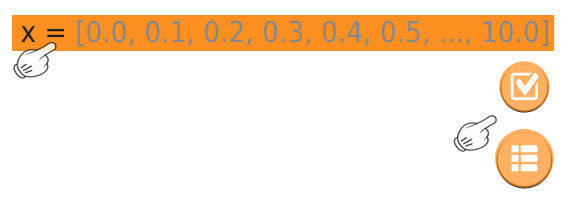
\includegraphics[resolution=320]{graphics/how_to_use_fig7.png} \end{tabular}\end{center}

Auch wird ein weiters Action Button
''Details'' angezeigt. Ein Tap auf
diesen Button öffnet das Dialogfenster
''Details'', wo Sie alle Vektorelemente
sehen können.

Bitte beachten Sie, dass die
Verwendung von drei oder mehr
intervallähnlichen Variablen im linken
Teil einer Ergebnisansicht in dieser
Version des Apps nicht gestattet ist.

\subsection{Funktionsgraph}

Das Funktionsgraph-Element bildet den
Graphen einer Funktion ab, die von
einem einzigen Argument abhängt. Um
einen Graphen zu erstellen, nutzen Sie
den ''Neu'' Button in der Menüleiste
oder ''Funktionsgraph hinzufügen''
Button in der Werkzeugleiste:
\begin{center}\begin{tabular}{c} 
\includegraphics[resolution=320]{graphics/how_to_use_fig8.png} \end{tabular}\end{center}

Eine Panel mit sechs lehre Feldern wird
erstellt. Die darzustellenden
Funktionen sollen im linken mittleren
Feld sein und das Funktionsargument im
mittleren unteren Feld.
\begin{center}\begin{tabular}{c} 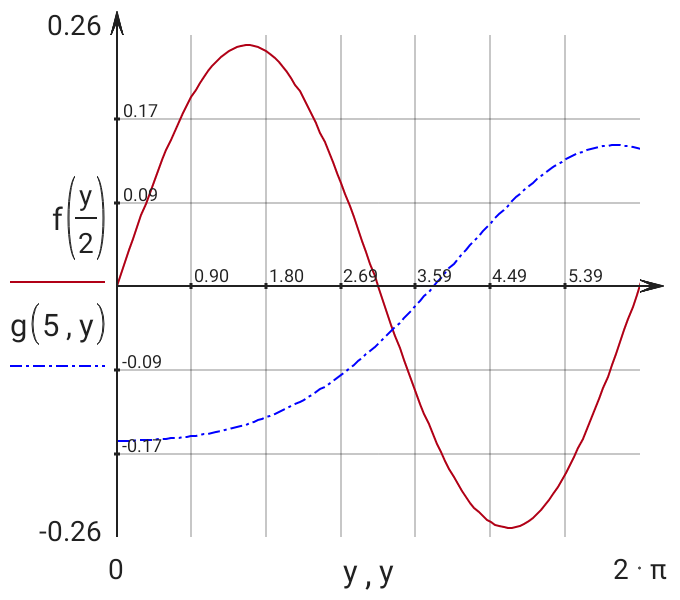
\includegraphics[resolution=320]{graphics/how_to_use_fig9.png} \end{tabular}\end{center}

Für mehr Details siehe das ''Plot einer
Funktion'' Beispiel des Hauptmenüs.

\subsection{3D Plot}

Das 3D Plot Element stellt Graphen
einer einzelnen Funktion dar, die von
zwei Argumenten abhängt. Um so einen
Plot zu erstellen, nutzen Sie den
''Neu'' Button in der Menüleiste oder
''3D Plot hinzufügen'' Button in der
Werkzeugleiste:
\begin{center}\begin{tabular}{c} 
\includegraphics[resolution=320]{graphics/how_to_use_fig10.png} \end{tabular}\end{center}
\begin{center}\begin{tabular}{cc}
  $x := \left[ -10,\, -9.5 \,..\, 10 \right]$ &
  $y := \left[ -10,\, -9.5 \,..\, 10 \right]$ \cr
\end{tabular}\end{center}
\begin{center}\begin{tabular}{c} 
\includegraphics[resolution=320]{graphics/how_to_use_fig11.png} \end{tabular}\end{center}

Fügen Sie im unteren Zentrum den
Funktionsname oder eine Gleichung ein,
die genau zwei zuvor definierte
Intervalle enthält. Sie können hier
auch ein Array benuzen:
\begin{center}\begin{tabular}{c} 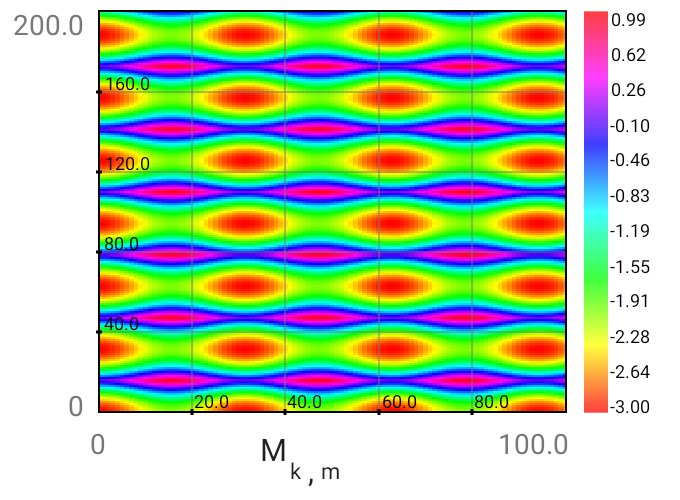
\includegraphics[resolution=320]{graphics/how_to_use_fig12.png} \end{tabular}\end{center}

Für mehr Details siehe ''3D Plot''
Beispiel im Hauptmenü.

\subsection{Textfragment}

Das Textfragment Element stellt
einfache Texte wie diesen hier da. Um
ein Textfragment hinzuzufügen, nutzen
Sie den ''Neu'' Button der Menüleiste
oder ''Textfragment hinzufügen'' Button
in der Werkzeugleiste:
\begin{center}\begin{tabular}{c} 
\includegraphics[resolution=320]{graphics/how_to_use_fig13.png} \end{tabular}\end{center}

Wenn Sie auf den Text lange gedrückt
halten, und dann den ganzen Text
mittels Kontexmenü  ''Alles auswählen''
markieren,  erscheint ein Action
Button ''Objekteinstellungen''.

Ein Tap auf diesen Button öffnet das
Dialogfenster ''Text-Einstellungen''.
Dort können Sie sowohl Textstil
ändern, als auch  die Numerierung
aktivieren.  Zum Beispiel, die
Überschriften im Dokument haben
Textstil ''Unterabschnitt'' und 
automatische Numerierung.

\subsection{Bild}

Sie können auch ein Bild aus einer
Datei hinzufügen. Nutzen Sie dafür den
Button ''Neu'' in der Menüleiste oder
den Button ''Bild aus Datei hinzufügen''
in der Werkzeugleiste:
\begin{center}\begin{tabular}{c} 
\includegraphics[resolution=320]{graphics/how_to_use_fig14.png} \end{tabular}\end{center}

Der Dialog ''Bildeinstellungen'' wird
geöffnet. Dort können Sie eine Datei
auswählen, in der das gewünschte Bild
abgespeichert ist und die gewünschte
Bildgröße festlegen.

Derzeit werden folgende Bildformate
unterstützt: png, bmp, gif, jpeg, svg.

Wenn das Kontrollkästchen ''In Dokument
einbetten'' im Dialog
''Bildeinstellungen'' aktiviert ist,
wird das Bild direkt in Ihr
Arbeitsblatt eingebettet. Das
Arbeitsblatt wird dann größer, kann
aber weiterhin benutzt werden, auch
wenn die ursprüngliche Datei mit dem
Bild gelöscht wurde.

Wenn das Kontrollkästchen ''In Dokument
einbetten'' nicht aktiviert ist, dann
wird das Arbeitsblatt mit dem Bild
verknüpft. Die Verknüpfung ist eine
Referenz auf die Datei außerhalb des
Arbeitsblattes. In diesem Fall müssen
beide Dateien (Arbeitsblatt und
Bilddatei) immer zusammen kopiert oder
verschoben werden.

Die Bildgröße kann mittels des
Dialogfensters ''Bildeinstellungen''
geändert werden. Wenn Sie auf dem Bild
lange gedrückt halten, erscheint ein
Action Button ''Objekteinstellungen''.
Ein Tap auf diesen Button öffnet
dieses Dialogfenster.
